\section{Introduction}

The purpose of this assignment was to get a solid understanding of how Linux device drivers work, how they can control hardware and how user applications can interact with hardware through them. An operating system provides a nice and clean software interface to hardware for user applications. Thus hiding the complexity of hardware, and making user application development a lot easier. But in order to support the vast amount of hardware available, the operating system needs device drivers control for their specific behaviour. The operating system provides the driver with an interface of functions that the driver can support(e.g. read, write, iseek), without caring how the driver implements them. So when a user application wishes to access hardware it invokes a system call. The kernel then calls the respective device driver (which resides in kernel space), which directly interact with the hardware. 

To get first hand experience with this; we were given the task of making a computer game for Linux, which should interact with a simple gamepad through a character device driver. We were provided with an EFM32GG development card, which had a simple gamepad attached(see figure \ref{figure_efm32gg}). The assignment tasks were the following\cite{compendium}:

\begin{enumerate}
	\item Configure and build the uClinux for the board.
	\item Make a driver for the buttons. It should be implemented as a kernel module. You are
	free to make the driver as you wish, but the minimum requirements are to support your
	needs for the game to work.
	\item Complete the game. Use the framebuffer driver for writing to the display. Use your own
	driver for reading the status of the buttons.
\end{enumerate}

Since the main foucs of the assigment was to learn how to make device drivers and how to make them interact with userspace, we decided to make a very simple game. In the game you control a shield which you are supposed to use to catch astroids that are falling down. The shield can be moved to the left or right by pressing button 1 and 3, respectively. See figure \ref{figure_game}. 

We ended up making three device drivers for the game: one driver for the gamepad, a driver that worked as a timer, and an attempted sound driver. The purpose of the gamepad driver was to read the status of the gamepad buttons. The timer driver was used to signal the game whenever it was supposed to update its screen (i.e. move the shield, add more astroids, move the astroid downward etc.). We also attempted making a sound driver, using the direct memory access (DMA), but we were unable to get to function properly. 

\begin{figure}[ht]
    \centering
      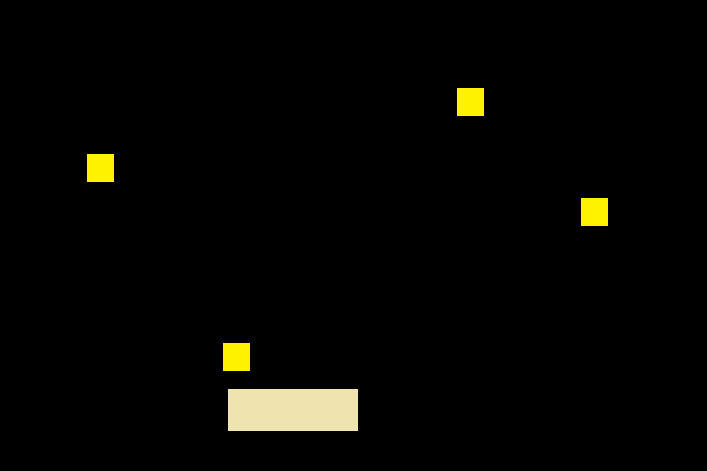
\includegraphics[width=9cm]{figures/game}
    \caption{The game. Move the shield to the left and right to prevent the yellow astroids from reaching the buttom.}
    \label{figure_game}
\end{figure}
 


\begin{figure}[ht]
    \centering
      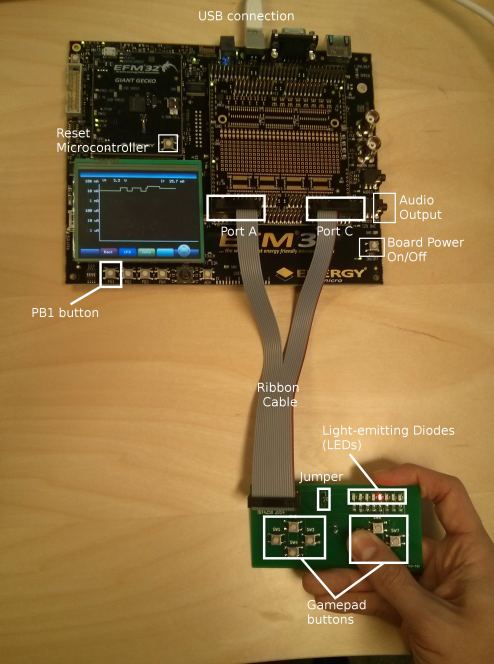
\includegraphics[width=9cm]{figures/efm32gg}
    \caption{The EFM32GG development card and gamepad\cite{compendium}}
    \label{figure_efm32gg}
\end{figure}
